\documentclass[a4]{jsbook}

\usepackage{ascmac}
\usepackage{here}
\usepackage{txfonts}
\usepackage{listings, jlisting}
\usepackage{fancyheadings}
\usepackage[dvipdfmx]{graphicx,color}
\usepackage{makeidx}
\renewcommand{\lstlistingname}{リスト}
\lstset{%language=Python,%
        basicstyle=\footnotesize,%
        commentstyle=\textit,%
        classoffset=1,%
        keywordstyle=\bfseries,%
	frame=tRBl,framesep=5pt,%
	showstringspaces=false,%
        numbers=left,stepnumber=1,numberstyle=\footnotesize%
	}%
\usepackage{ascmac}


\setlength{\textwidth}{\fullwidth}
\setlength{\evensidemargin}{\oddsidemargin}

\makeatletter
\def\ps@plainfoot{%
  \let\@mkboth\@gobbletwo
  \let\@oddhead\@empty
  \def\@oddfoot{\normalfont\hfil-- \thepage\ --\hfil}%
  \let\@evenhead\@empty
  \let\@evenfoot\@oddfoot}
\let\ps@plain\ps@plainfoot
\makeatother
\pagestyle{plain}

\setlength\footskip{2\baselineskip}
\addtolength{\textheight}{-2\baselineskip}


\lhead{Usage of fancyheading.sty}
\chead{}
\rhead{\roman{page}}
\lfoot{}
\cfoot{Copyrights (C) 1999 TAMAYA All Rights Reserved.}
\rfoot{}
\pagestyle{fancy}


\title{...}
\author{...}
\date{\today}

\begin{document}
%
\maketitle
\frontmatter
%
\addcontentsline{toc}{chapter}{概要}
\include{abstract}
\tableofcontents
%
%

\mainmatter
\chapter{Title for Chapter1}%

\begin{abstract}

\begin{figure}[htbp]
 \begin{center}
 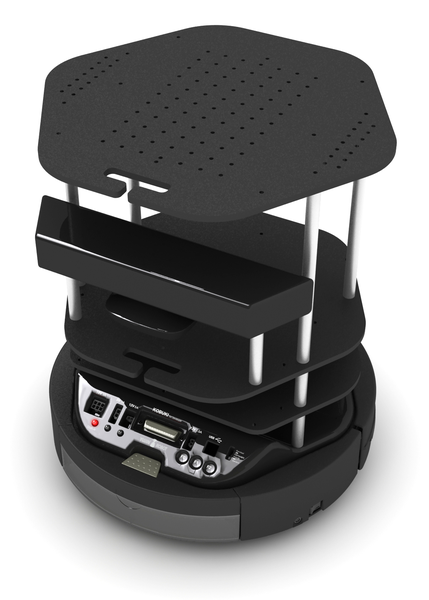
\includegraphics[width=5cm,clip]{Back_grande.png}
 \end{center}
 \caption{テスト図}
\end{figure}

ROSで地図を作って、経路探索するまでの手順
\end{abstract}

\section{はじめのセクション}

ROSで地図を作って、経路探索するまでの手順
ROSで地図を作って、経路探索するまでの手順
ROSで地図を作って、経路探索するまでの手順
ROSで地図を作って、経路探索するまでの手順
ROSで地図を作って、経路探索するまでの手順
ROSで地図を作って、経路探索するまでの手順
ROSで地図を作って、経路探索するまでの手順


\index{さくいんさんぷる1@索引サンプル1}%



\chapter{sadsadas}
\begin{lstlisting}[caption=キャプション,label=ラベル]
# -*- coding: utf-8 -*-
print u"モジュールのロード"
def test():
    print u"関数:testを呼び出しました"

if __name__ == "__main__":
    print "python-izm"
#   print "パイソンイズム"
    test()

\end{lstlisting}


\begin{shadebox}
{\tt
\$ sudo apt-get install ros-hydro-aaaa\\
\$ sudo apt-get install ros-hydro-aaaa
}
\end{shadebox}



\appendix
%
\include{appendixA}
\include{appendixB}
%
\chapter*{謝辞}
\addcontentsline{toc}{chapter}{謝辞}
...
...
%
%
\include{biblography}
%
%
\newpage
\printindex


\end{document}
